\section{Introduction}

With the recent rise in sales in the smartphone/PDA market
and the recent launch of several tablet form-factor devices (Tablet PCs, Apple iPad, Amazon's Kindle), users increasingly use medium sized touch screens. These screens offer
more screen space than a traditional phone, and can arguably be more
effective in text-input tasks. Due to increased size and weight,
however, these devices require specific postures from the users to be
able to input text. Direct touch or pen input causes the additional issue of occlusion \todo{cite Vogel}. Therefore, text entry on such devices continues to be a difficult problem.

Moreover, the tablet form-factor introduces two problems for the user.
First, since a tablet is very portable, it is an ideal device for use
while mobile (e.g. actually moving, rather than nomadic, meaning in
different places, but mostly stationary).  Doctors in a busy hospital,
commuters standing on a train and TV producers on location at a shoot
are all examples of users who would benefit from using a computing
device while standing, walking or sitting and briefly holding their
device.
\begin{figure}
    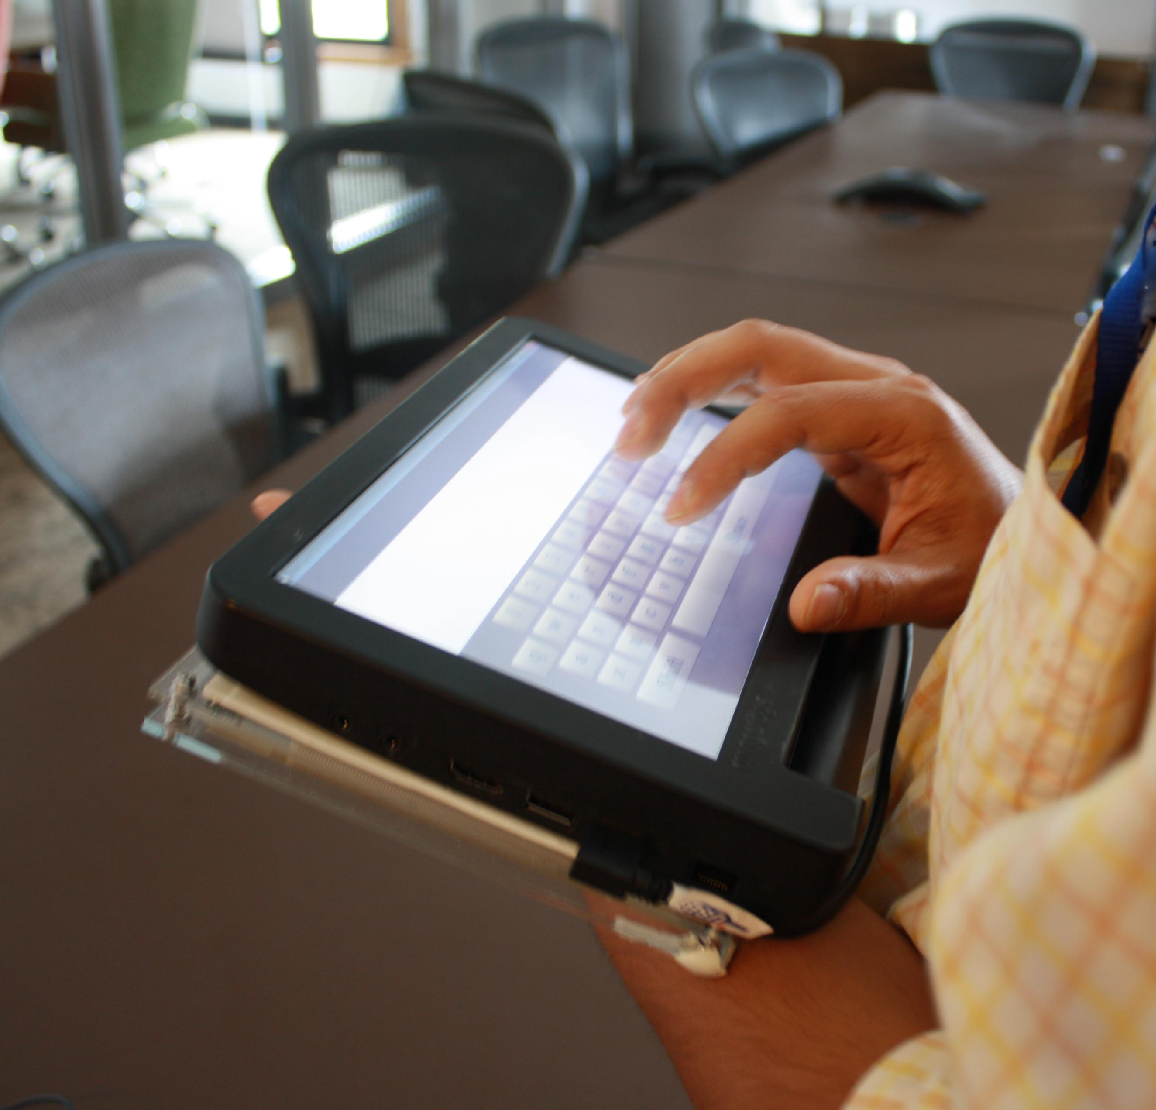
\includegraphics[scale=0.35]{Figures/device_hold.pdf} 
  	\caption{A user holding a foot-scale device and trying to enter text. It can be seen how this is unstable and unnatural.}
    \label{fig:device_hold}
\end{figure}
Unlike a mobile phone, however, a larger (e.g. 7+ inches wide)
keyboard (soft or otherwise) does not work well with two thumbs
because of the relatively large distance that the thumbs must travel
to reach the appropriate keys.   The weight of the device compounds
the problem of typing by straining the hands to support the device
while making precise movements to position the thumbs over the proper
keys. While standing, many users resort to a different pose, in which
one arm supports the device while the other hand types with a single
finger (Figure~\ref{fig:device_hold}). 

A second difficulty, common to all soft keyboards, arises because the
fingers do not receive any tactile feedback as to their position on
the keyboard.  Unlike a physical keyboard in which the keys have
ridges that delineate their boundaries, a soft keyboard often requires
the user to look at the keyboard to ensure that they are activating
the correct keys.  Looking at the keys while typing is distracting,
requires many eye shifts (since the user must also verify on the
screen that what they are typing is correct), and requires a higher
cognitive load than "touch-typing", since the user must visually
process each key tap.  This can be alleviated to some extent by
providing haptic feedback when a key is activated, but this provides
only limited improvement.

At the same time, there has recently been a push in the industry for
devices with "backside" input, in which the device has a touch input
device or keyboard on the opposite side of the main display. Notion
Ink's Adam PC has a backside trackpad [1]. Samsung and Toshiba have
also been making effort towards backside touch input
\todo{citations}. As manufacturers start to include backside input in their devices, we have an opportunity to take advantage of this new input modality to improve the users speed, a
ccuracy and comfort while entering text on their "foot-scale" devices.  A "natural" method of holding such a device is to have hands on both the sides with fingers wrapped around o
n the back.
(Figure~\ref{fig:natural})

Users can take advantage of devices with back-of-device input in a variety
of different scenarios. When the user is stationary and visually
focused, they are more flexible in the pose that they use, and a
traditional QWERTY keyboard may work in this scenario, although the
complicated visual feedback cycle still has a high cognitive load for
the user, and requires precise gross motor movements, limiting their speed an accuracy. 

Another scenario to consider is when the user is mobile but still
visually focused, but occasionally losing focus while entering
text(for example while commuting on a train).  With a QWERTY keyboard,
users have to orient themselves again after each lapse. Such scenarios
benefit from mechanisms that don't require the user to re-orient
themselves when they lose focus.  Scenarios in which the user is only
intermittently focused, such as when they are walking require
mechanisms that help the user memorize certain set patterns and
configurations, that they could later replicate even without looking
at the interface. 

In this paper we present text-input mechanisms that could be tested on devices with back-of-device touch input. The goal is to provide mechanisms that could allow users to enter text on devices with larger screens and back-of-device touch input in a way that eliminates the problems of occlusion of screen space inherent to touch and pen input, and uses the established effectiveness of vertical movements on back-of-device touch input \todo{cite Wobbrock} by giving freedom of movement to multiple fingers. We acknowledge the fact that there have been efforts in the recent past \todo{cite Reartype and LucidTouch} that try do the same, but we want to investigate the solutions to the problem of text-entry in the absence of additional hardware like hover sensing (LucidTouch) and discrete physical keys (RearType). We understand that our implementation can be viewed as sub-optimal in the view of these recent contributions, but we wanted to experiment with mechanisms that are implementable on existing devices with back-of-device touch input without adding extra hardware.

We have designed a chording-based touch input mechanism specifically
for devices with a back-of-device touch input.  This mechanism that shows
promise in the scenarios described above.  Figure~\ref{fig:natural}
illustrates that entering text on the back of the device results in a
more natural, comfortable and stable pose than the commonly adopted
pose shown in Figure~\ref{fig:device_hold}.  We designed the mechanism
to use large, relatively inaccurate finger movements as the building
block for chords.  This allows the user to exploit proprioceptive
feedback (e.g. feedback from in the nervous system of the hands that
signals the relative positions of the fingers to one another) to
increase their speed and accuracy by reducing or eliminating the
visual feedback required to enter text. 

\begin{figure*}
    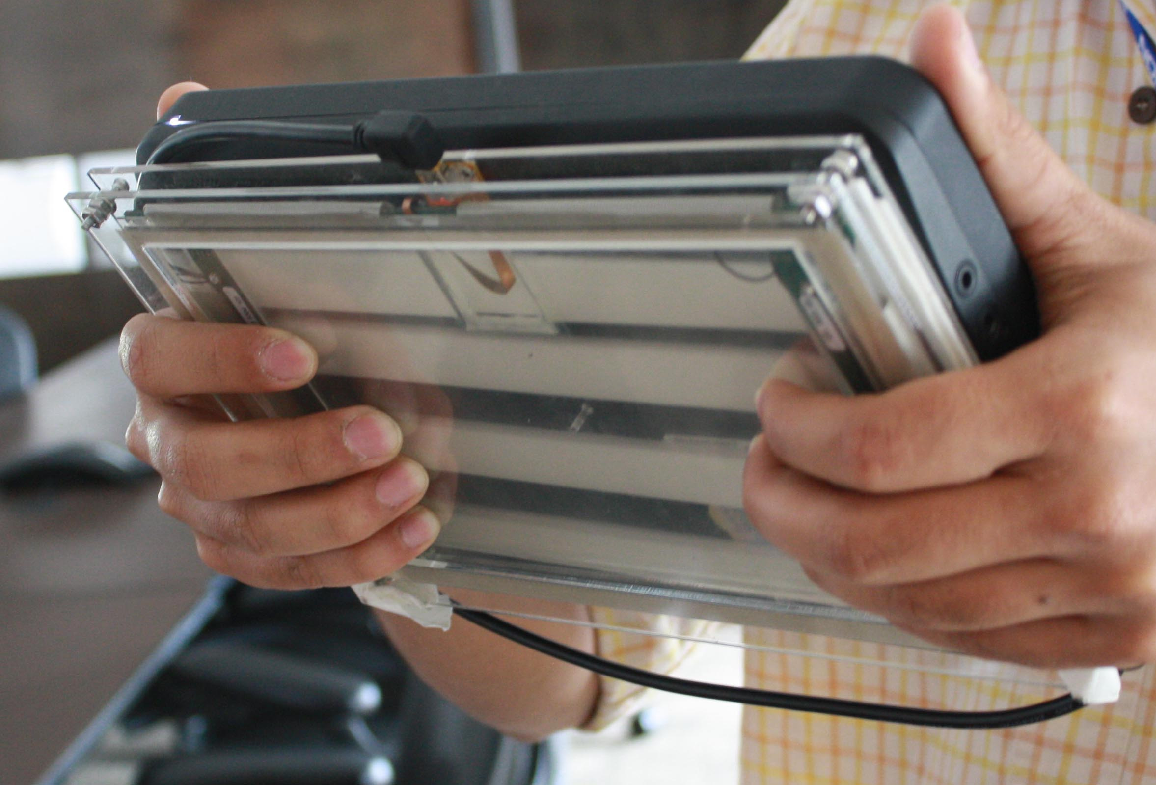
\includegraphics[scale=0.43]{Figures/natural1.pdf} 
     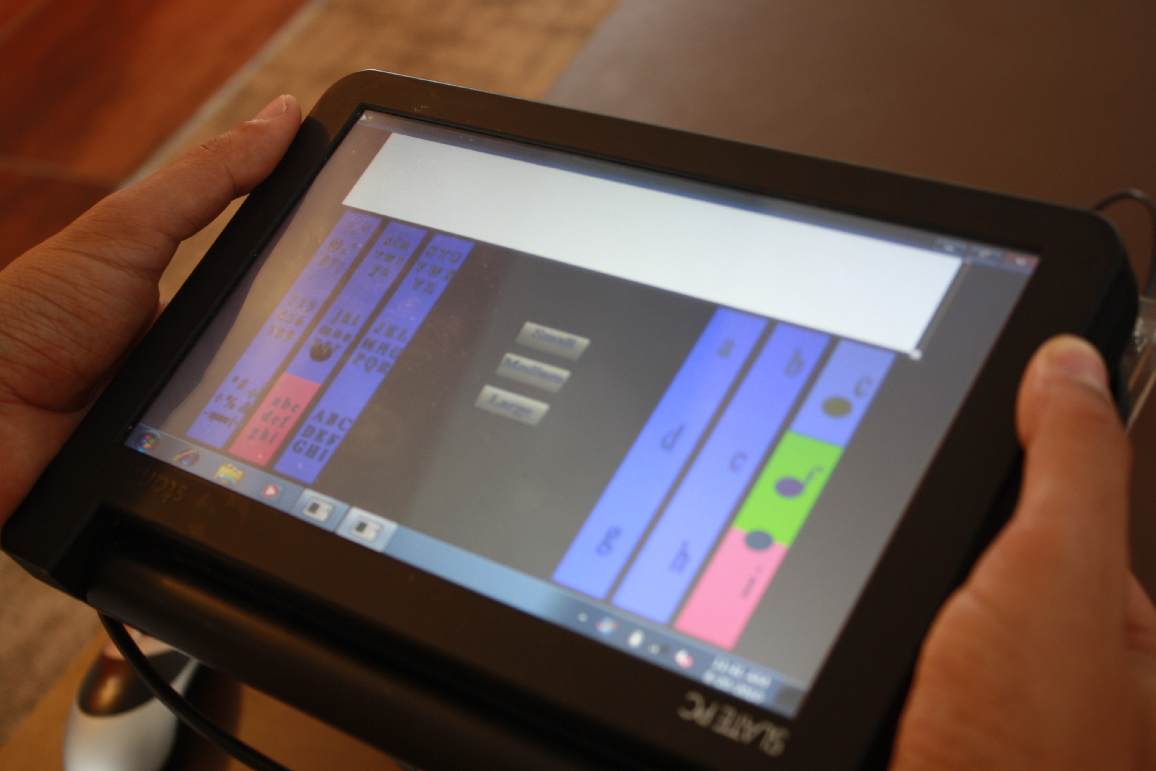
\includegraphics[scale=0.43]{Figures/natural2.pdf} 
     \caption{A user holding a mobile device with medium-sized touch
       screen in a natural and stable posture. The user is able to see
       his finger positions on the screen on the front. The figure
       also shows our hardware prototype with a multitouch screen on
       the rear of a Slate PC.}
        \label{fig:natural}
\end{figure*}

In this paper we detail our initial quantitative and qualitative investigation of this new mechanism. However, just like in the case of other exploratory works \todo{cite RearType} our focus for this phase of experimentation was to determine if users find such input mechanisms usable or frustrating. There can also be additional concerns with use of back-of-device touch input, like minimized grip stability. In view of such issues it was necessary to investigate the user perception around back-of-device text-input. To capture that we use the NASA Task Load Index (TLX) and present an analysis of the reported user experience. Using a hardware prototype with a multitouch input on both the back and the front of the device, we compare the performance of the novel chording mechanism and a backside QWERTY with a standard soft QWERTY keyboard on the front or the back of the device in a controlled, 36-user study.  Based on these results, we recommend further avenues for research and modifications to the current mechanism which we believe will results in better performance.
